\subsection{Flyweight}
\subsubsection{Định nghĩa}
Mẫu thiết kế Flyweight là một mẫu thiết kế trong đó chúng ta tối ưu hóa việc sử dụng bộ nhớ bằng cách chia sẻ một số lượng lớn các đối tượng nhỏ chung. Nó giúp giảm sự lặp lại dữ liệu và tiết kiệm tài nguyên bộ nhớ bằng cách chia sẻ chúng giữa nhiều đối tượng.
\subsubsection{Cách sử dụng}
Flyweight thường được sử dụng trong các trường hợp sau:
\begin{itemize}
    \item Khi bạn có một số lượng lớn các đối tượng và việc lưu trữ tất cả chúng trong bộ nhớ sẽ tốn rất nhiều tài nguyên.
    \item Khi các đối tượng có các thuộc tính giống nhau và có thể chia sẻ được giữa nhiều đối tượng.
    \item Khi bạn muốn giảm bộ nhớ sử dụng bằng cách chia sẻ dữ liệu chung giữa các đối tượng.
\end{itemize}
\subsubsection{Cấu trúc}
Các thành phần chính:
\begin{itemize}
    \item Class Flyweight chứa phần trạng tháo đầu của đối tượng có thể được chia sẽ giữa nhiều đối tượng. 
    \item Class Context chứa trạng thái được truyền cho các phương thưc flyweight.
    \item Flyweight Factory để quản lí một nhóm các Flyweight hiện có.
\end{itemize}
\begin{center}
    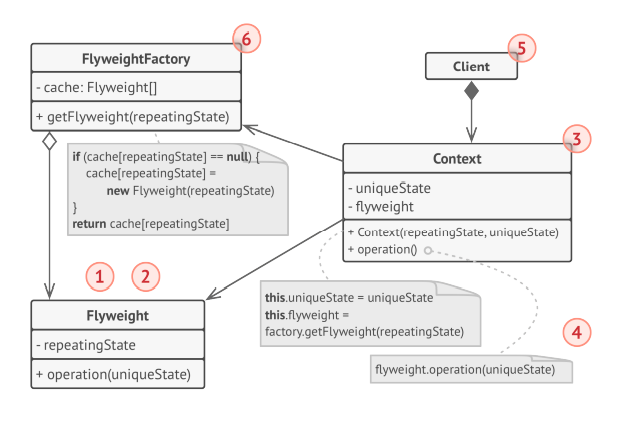
\includegraphics[scale=0.6]{image/structural/flyweight.png}
\end{center}
\begin{itemize}
    \item Về bản chất flyweight là gôm các điểm chung của các object thành 1 thành phần và kết hợp với các đối tượng sử dụng bộ đặc điểm chung đó.
\end{itemize}
\subsubsection{Ưu điểm và Nhược điểm}
Ta có các ưu nhược điểm sau:\\
Ưu điểm:
\begin{itemize}
    \item Tiết kiệm tài nguyên bộ nhớ bằng cách chia sẻ dữ liệu chung giữa các đối tượng.
    \item Giảm số lương đối tượng được tạo ra bằng cách chia sẻ đối tượng. Vì vậy tiết kiệm bộ nhớ và các thiết bị lưu trữ cần thiết.
\end{itemize}
Nhược điểm:
\begin{itemize}
    \item Cần quản lý sự chia sẻ dữ liệu một cách cẩn thận để đảm bảo tính toàn vẹn dữ liệu giữa các đối tượng.
    \item Việc chia sẻ dữ liệu có thể làm cho việc xử lý và quản lý phức tạp hơn.
\end{itemize}
\subsubsection{Code Example}
\begin{itemize}
    \item Ta có class Hình vuông và một nhà máy để tạo ra các hình vuông dựa vào vài yếu tố.
\end{itemize}
\begin{lstlisting}
#include <iostream>
#include <vector>
#include <map>

// Flyweight: Square
class Square {
private:
    std::string color;
    int size;

public:
    Square(const std::string& color, int size) : color(color), size(size) {}

    void draw(int x, int y) {
        std::cout << "Draw square: Color " << color << ", Size " << size << ", Position (" << x << ", " << y << ")" << std::endl;
    }
};

// Flyweight Factory: Manages shared Square objects
class SquareFactory {
private:
    std::map<std::string, Square*> squares;

public:
    Square* getSquare(const std::string& color, int size) {
        std::string key = color + "_" + std::to_string(size);
        if (squares.find(key) == squares.end()) {
            squares[key] = new Square(color, size);
        }
        return squares[key];
    }
};

// Client: Uses Square objects
int main() {
    SquareFactory squareFactory;

    std::vector<std::pair<int, int>> positions = { {0, 0}, {10, 5}, {3, 8}, {7, 2} };

    Square* blueSquare = squareFactory.getSquare("Blue", 10);
    Square* redSquare = squareFactory.getSquare("Red", 10);

    for (const auto& pos : positions) {
        blueSquare->draw(pos.first, pos.second);
        redSquare->draw(pos.first + 1, pos.second + 1);
    }

    return 0;
}

\end{lstlisting}
Ở hàm main, ta gọi một nhà máy sản xuất hình vuông và sản xuất 2 loại hình vuông xanh đỏ trên một bộ số có sẵn.\\
\newline
\textbf{Kết quả:}
\begin{lstlisting}
Draw square: Color Blue, Size 10, Position (0, 0)
Draw square: Color Red, Size 10, Position (1, 1)
Draw square: Color Blue, Size 10, Position (10, 5)
Draw square: Color Red, Size 10, Position (11, 6)
Draw square: Color Blue, Size 10, Position (3, 8)
Draw square: Color Red, Size 10, Position (4, 9)
Draw square: Color Blue, Size 10, Position (7, 2)
Draw square: Color Red, Size 10, Position (8, 3)
\end{lstlisting}
\subsubsection{Các Pattern liên quan}
\begin{itemize}
    \item Sử dụng các node lá của Composite nếu nó có thuộc tính cung có thể cài đặt theo kiểu Flyweight.
    \item Facade có thể kết hợp với Flyweight do flyweight là chia đối tượng lớn ra nhiều đối tượng nhỏ còn facade là gôm tất cả đối tượng nhỏ thành đối tượng lớn.
\end{itemize}